\documentclass[compress,aspectratio=1610]{beamer}

\usepackage[ngerman]{babel}
\usepackage[english]{isodate}
\usepackage{amssymb}
\isodate
\usepackage{multicol}
\usepackage{tikz}
\usepackage{xcolor}
\usetikzlibrary{matrix,calc}
\usepackage{minted}

%% THEMES : vertex or green %%
%% OPTIONS: vertex & green %%
%%          [bincount] o. [bincount, totalframes]
%%          [hexcount] o. [hexcount, totalframes]
%%          []         o. [totalframes]
%% OPTIONS: vertex %%
%%          [dark] 
%%          [simplefootline]

%\usetheme[simplefootline, bincount]{vertex}
%\usetheme[totalframes]{green}
\usetheme[hexcount]{vertex}

\usepackage{blkarray}
\linespread{1.1}

\title{Quantencomputer}
\subtitle{Werkzeuge f\"ur die Algorithmenimplementierung}
\date{\today}
\author{Timo Grautst\"uck}
\institute[]{
  Fachhochschule Dortmund \\
  FB 10: Informationstechnik
}
\begin{document}

\maketitle

\section*{Inhalt}
\begin{frame}
  \frametitle{Inhalt}
  \centering
  \tableofcontents[hideallsubsections]
\end{frame}

\section{Grundlagen Quantencomputer}
\begin{frame}{Warum Quantencomputer?}
  \begin{minipage}{0.6\textwidth}
    \begin{itemize}
    \item Shors Algorihmus: $\mathcal{O}((\log n)^3)$
    \item Grover Algorithmus: $\mathcal{O}(\sqrt{N})$
    \item Quantenkryptographie: key exchange problem
    \item \textbf{Quanten\"uberlegenheit \textit{(Quantum Supremacy)}}
    \end{itemize}
  \end{minipage}
  \hfill
  \begin{minipage}{0.3\textwidth}
    \begin{figure}[h]
    \centering
    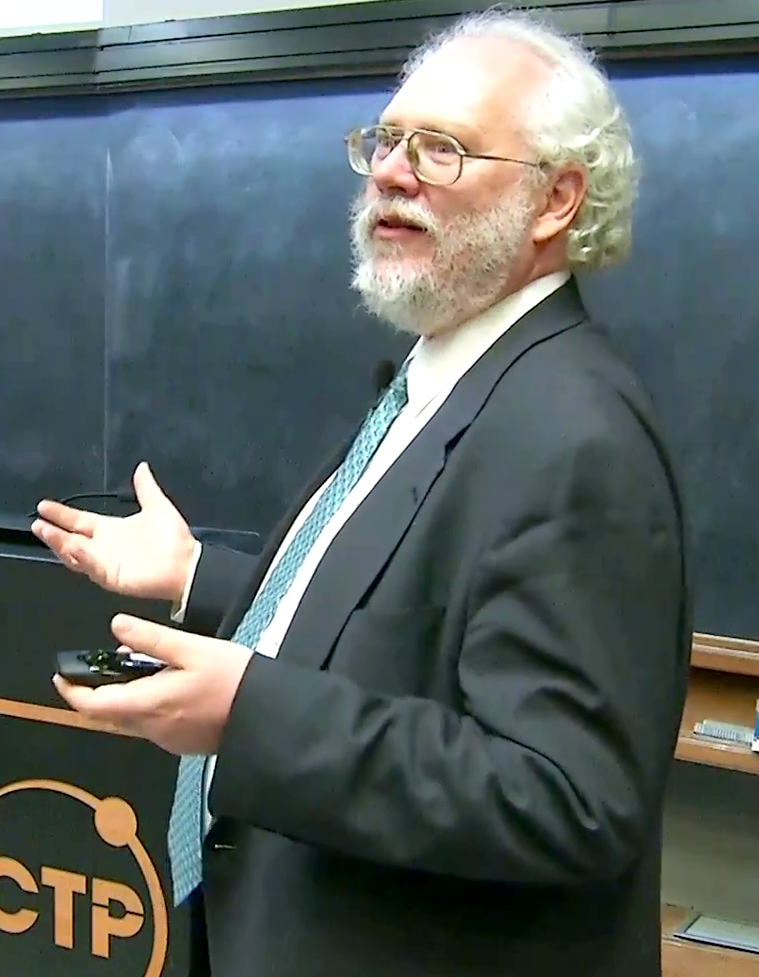
\includegraphics[width=1\textwidth]{figures/Peter_Shor_2017.png}
    \caption{Peter Shor 2017}
    \end{figure}
  \end{minipage}
  \vfill
  \tiny{Bildquelle (wikimedia): \url{https://commons.wikimedia.org/wiki/File:Peter_Shor_2017_Dirac_Medal_Award_Ceremony.png}}
\end{frame}

\begin{frame}{Quanten supremacy}
  \begin{minipage}{0.45\textwidth}
    \centering
    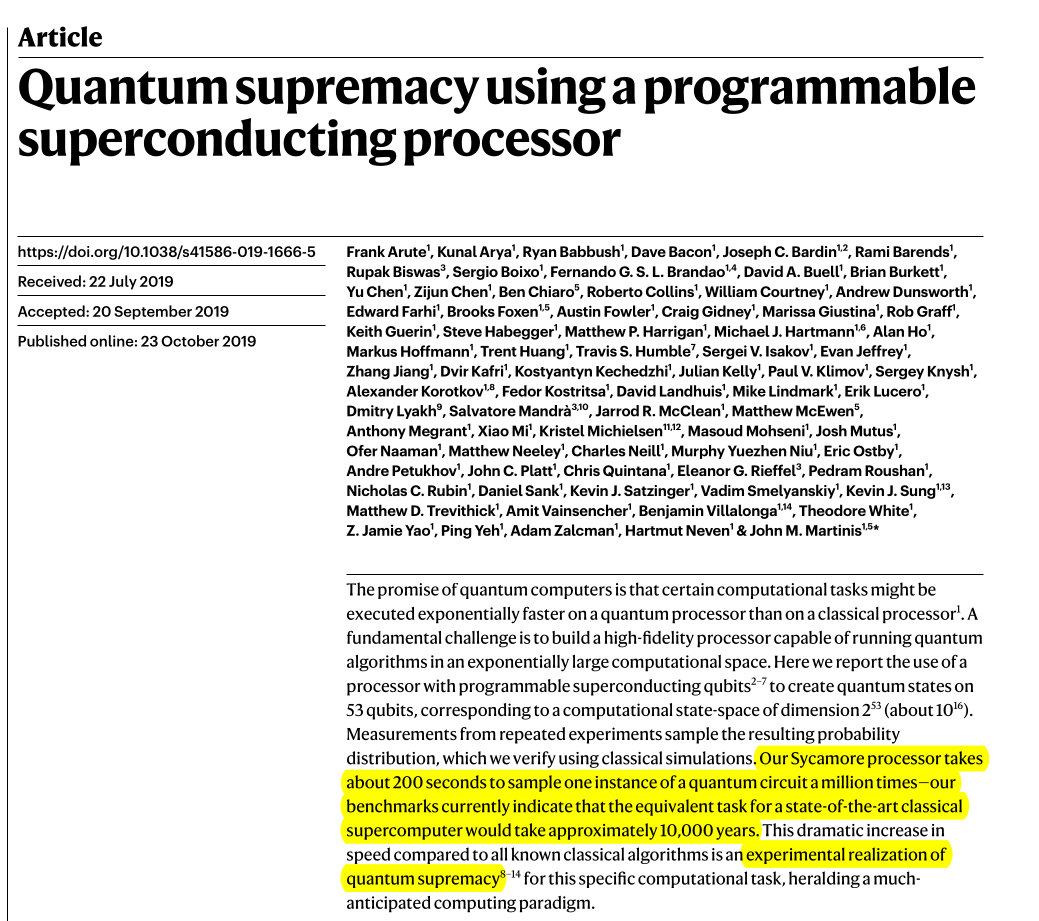
\includegraphics[width=1.1\textwidth]{figures/Quantum-Supremacy.png}
  \end{minipage}
  \hfill
  \begin{minipage}{0.45\textwidth}
    \centering
    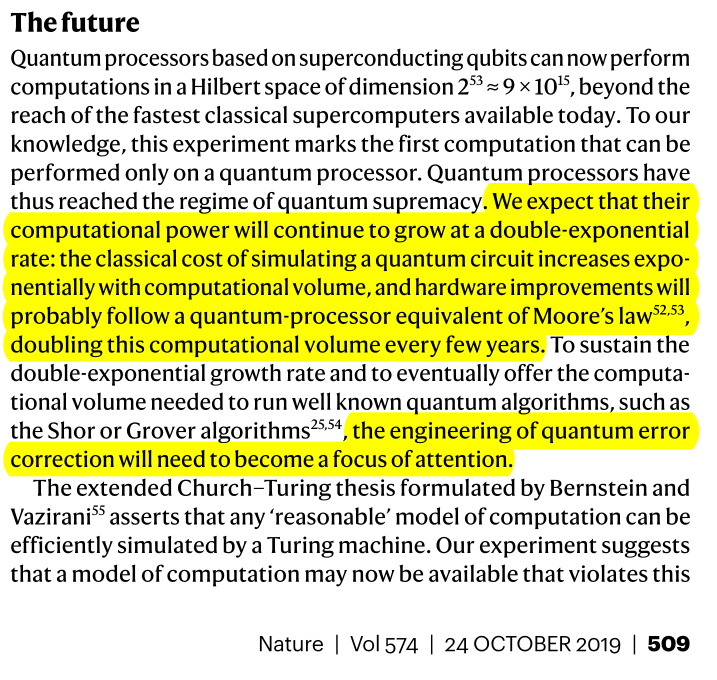
\includegraphics[width=0.7\textwidth]{figures/The-Future.png}
  \end{minipage}
  \vfill
  \tiny{\href{https://www.nature.com/articles/s41586-019-1666-5}{Quantum supremacy using a programmable superconducting processor} \cite{Arute2019}}
\end{frame}    


\begin{frame}{Quantenbits I}
  \begin{block}{Basiszust\"ande}
    \begin{equation}\nonumber
      |0\rangle = \begin{bmatrix}
        1 \\
        0 \\
      \end{bmatrix}
      \,\,\, \,\,\,
      |1\rangle = \begin{bmatrix}
        0 \\
        1 \\
      \end{bmatrix}
    \end{equation}
  \end{block}
  \begin{block}{Zweizustandssystem}
    Kann sich in einer Superposition der Basiszust\"ande befinden:
    \begin{equation}\nonumber
      \begin{gathered}
        |\psi\rangle = \alpha |0\rangle+\beta |1\rangle = \begin{bmatrix}
          \alpha \\
          \beta \\
        \end{bmatrix} \qquad \alpha, \beta \in \mathbf{C} \\[0.5em]
        |\psi\rangle = \cos\left(\frac{\theta}{2}\right)|0\rangle+e^{i\phi}\sin\left(\frac{\theta}{2}\right)|1\rangle \qquad \theta, \phi \in \mathbf{R}
      \end{gathered}
    \end{equation}
  \end{block}
  \begin{itemize}
  \item $\phi$ und $\theta$ sind Kugelkoordinaten, der Radius $r = 1$
  \end{itemize}
\end{frame}

\begin{frame}{Quantenbits II}
  \begin{minipage}{0.45\textwidth}
    \begin{block}{Normalisierung}
      \begin{equation}\nonumber
        \begin{gathered}
          \langle \psi | \psi \rangle = 1 \\
          \Rightarrow |\alpha|^2 +|\beta|^2 = 1
        \end{gathered}
      \end{equation}
    \end{block}
    \begin{block}{Beispiel: \color{white}\phi=0 und \theta=\pi/2}
      \begin{equation}\nonumber
        \begin{gathered}
          |\psi\rangle = \cos\left(\frac{\pi}{4}\right)|0\rangle+e^{i0}\sin\left(\frac{\pi}{4}\right)|1\rangle \\[0.5em]
          \Rightarrow |\psi\rangle = |+\rangle = \frac{1}{\sqrt{2}}\left(|0\rangle+|1\rangle\right)
        \end{gathered}
      \end{equation}
    \end{block}
  \end{minipage}
  \hfill
  \begin{minipage}{0.45\textwidth}
    \begin{figure}
      \centering
      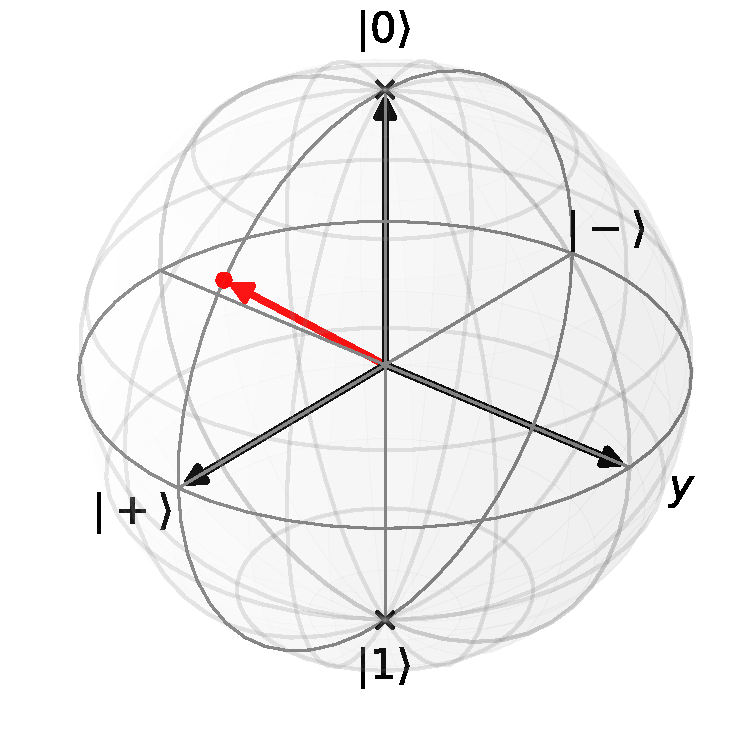
\includegraphics[width=0.8\textwidth]{~/sciebo/Projektarbeit-2/ausarbeitung/figures/blochsphere.pdf}
      \caption{Bloch-Kugel \textit{(Blochsphere)}}
    \end{figure}
  \end{minipage}
\end{frame}

\begin{frame}{Quantenbits III}
  \begin{block}{Quantenregister}
    \begin{itemize}
    \item $n$ Qubits besitzten $2^n$ Wahrscheinlichkeitsamplituden 
    \end{itemize}
    \begin{equation}\nonumber
      |\psi \rangle = \alpha_{00} |00\rangle + \alpha_{01} |01\rangle + \alpha_{10} |10\rangle + \alpha_{11} |11\rangle = \begin{bmatrix} \alpha_{00} \\ \alpha_{01} \\ \alpha_{10} \\ \alpha_{11} \end{bmatrix}
    \end{equation}
    \begin{itemize}
    \item K\"onnen durch Produkte der Basiszust\"ande beschreiben werden
    \end{itemize}
    
    \begin{equation}\nonumber
      \begin{aligned}
        |0\rangle\otimes |0\rangle = |00\rangle = \begin{bmatrix}1 \times \begin{bmatrix} 1\\0\end{bmatrix}\\[1em] 0 \times \begin{bmatrix} 1\\0\end{bmatrix}\end{bmatrix} = \begin{bmatrix} 1 \\ 0 \\ 0 \\ 0\end{bmatrix}
      \end{aligned}
    \end{equation}
  \end{block}
\end{frame}

\begin{frame}{Quantengatter I}
    \begin{itemize}
    \item Manipulation von Qubits
    \item Quantengatter die auf $n$ Bits operieren sind unit\"are $2^n\times 2^n$-Matrizen
    \item Für diese Matrizen existieren Eigenvektoren 
    \end{itemize}
    \begin{minipage}{0.45\textwidth}
      \begin{block}{Unit\"ar}
        \begin{equation}\nonumber
          \boxed{I = A^{\dagger}A} \qquad A^{\dagger} = A^{\ast T}
        \end{equation}
      \end{block}
      \begin{block}{Eigenvektor \& Eigenwert}
        $$A|\psi\rangle = \lambda |\psi\rangle = e^{2\pi i \theta}|\psi\rangle$$
      \end{block}
    \end{minipage}
    \hfill
    \begin{minipage}{0.45\textwidth}
      \begin{block}{Beispiel: X- \& H-Gatter}
        \begin{equation}\nonumber
          \begin{aligned}
          X &= |0\rangle\langle1|+|1\rangle\langle0| =
          \begin{bmatrix}
            0 & 1 \\
            1 & 0
          \end{bmatrix}\\[1em]
          H &= |0\rangle\langle+|+|1\rangle\langle-| = \frac{1}{\sqrt{2}}
          \begin{bmatrix}
            1 & 1 \\
            1 & -1
          \end{bmatrix}
          \end{aligned}
        \end{equation}
      \end{block}
    \end{minipage}
\end{frame}

\begin{frame}{Quantengatter II - \textit{(Pauligatter)}}
  \begin{table}[h] 
    \begin{tabular}{@{\hspace{0.7cm}}c@{\hspace{0.7cm}} | @{\hspace{0.7cm}}c@{\hspace{0.7cm}} | @{\hspace{0.8cm}}c@{\hspace{0.7cm}}}
      \hline 
      Matrix & Schaltungssymbol & Wahrheitstabelle \\
      \hline & \\
      $X = \begin{bmatrix} 0 & 1 \\ 1 & 0 \end{bmatrix}$ &
      \raisebox{-.3\height}{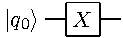
\includegraphics[width=0.2\textwidth]{~/sciebo/Projektarbeit-2/ausarbeitung/figures/pauli_x.pdf}} &
      \begin{tabular}{|c||c||c|}
        \hline
        Fall & $|q\rangle$ & $X|q\rangle$ \\
        \hline \hline 
        1 & $|0\rangle$ & $|1\rangle$ \\
        2 & $|1\rangle$ & $|0\rangle$ \\
        \hline
      \end{tabular} \\&\\

      %%%%%%%%%%%%%%%%%%%%%%%%%%%%%%%%%%%%%%%%%%%%%%%%%%%%%%%%%%%%%%

      $Y = \begin{bmatrix} 0 & -i \\ i & 0 \end{bmatrix}$ &
      \raisebox{-.3\height}{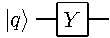
\includegraphics[width=0.2\textwidth]{~/sciebo/Projektarbeit-2/ausarbeitung/figures/pauli_y.pdf}} &
      \begin{tabular}{|c||c||c|}
        \hline
        Fall & $|q\rangle$ & $Y|q\rangle$ \\
        \hline \hline 
        1 & $|0\rangle$ & $i|1\rangle$ \\
        2 & $|1\rangle$ & $-i|0\rangle$ \\
        \hline
      \end{tabular} \\&\\

      %%%%%%%%%%%%%%%%%%%%%%%%%%%%%%%%%%%%%%%%%%%%%%%%%%%%%%%%%%%%%%

      $Z = \begin{bmatrix} 1 & 0 \\ 0 & -1 \end{bmatrix}$ &
      \raisebox{-.3\height}{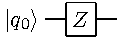
\includegraphics[width=0.2\textwidth]{~/sciebo/Projektarbeit-2/ausarbeitung/figures/pauli_z.pdf}} &
      \begin{tabular}{|c||c||c|}
        \hline
        Fall & $|q\rangle$ & $Z|q\rangle$ \\
        \hline \hline 
        1 & $|0\rangle$ & $|0\rangle$ \\
        2 & $|1\rangle$ & $-|1\rangle$ \\
        \hline
      \end{tabular} \\&\\
      \hline
    \end{tabular}
    \caption{Pauli Gatter}
  \end{table}
\end{frame}

\begin{frame}{Quantengatter III - \textit{(kontrollierte Gatter)}}
  \begin{minipage}{0.6\textwidth}
    \begin{itemize}
    \item Alle Gatter k\"onnen kontrolliert auf $n$ Qubits angewandt werden
    \item Ein Zielqubit und $n-1$ kontrollierende Qubits
    \item Um eine Transformation auf einem Zielbit auszuf\"uhren, m\"ussen sich alle kontrollierenden Bits im Zustand $|1\rangle$ befinden
  \end{itemize}
  \end{minipage}
  \hfill
  \begin{minipage}{0.3\textwidth}
    \begin{figure}
      \centering
      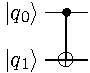
\includegraphics[width=0.7\textwidth]{~/sciebo/Projektarbeit-2/ausarbeitung/figures/cnot.pdf}
      \caption{Kontrolliertes-Nicht-Gatter}
    \end{figure}
  \end{minipage}
  \begin{block}{Beispiel: CNOT}
    $$CX_{01} = |0\rangle\langle0|\otimes I +|1\rangle\langle1|\otimes X =
    \begin{bmatrix}
      1 & 0 & 0 & 0 \\
      0 & 1 & 0 & 0 \\
      0 & 0 & 0 & 1 \\
      0 & 0 & 1 & 0 \\
    \end{bmatrix}$$
  \end{block}
\end{frame}

\begin{frame}{Quantengatter IV - \textit{(Toffoli-Gate)}}
  \begin{table}[h]
    \begin{tabular}{c|c|c}
      \hline 
      Matrix & Schaltungssymbol & Wahrheitstabelle \\
      \hline & \\
      %%%%%%%%%%%%%%%%%%%%%%%%%%%%%%%%%%%%%%%%%%%%%%%%%%%%%%%%%%%%%%

      $CCX_{012} = \begin{bmatrix} I_2 & 0_2 & 0_2 & 0_2 \\ 0_2 & I_2 & 0_2 & 0_2 \\ 0_2 & 0_2 & I_2 & 0_2 \\ 0_2 & 0_2 & 0_2 & X \end{bmatrix}$ &
      \raisebox{-.5\height}{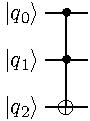
\includegraphics[width=0.16\textwidth]{~/sciebo/Projektarbeit-2/ausarbeitung/figures/toffoli.pdf}} &
      \begin{tabular}{|c||c||c|}
        \hline
        Fall & $|q_0 q_1 q_2 \rangle$ & $CCX_{012}|q_0 q_1 q_2\rangle$ \\
        \hline \hline 
        1 & $|000\rangle$ & $|000\rangle$ \\
        2 & $|001\rangle$ & $|001\rangle$ \\
        3 & $|010\rangle$ & $|010\rangle$ \\
        4 & $|011\rangle$ & $|011\rangle$ \\
        5 & $|100\rangle$ & $|100\rangle$ \\
        6 & $|101\rangle$ & $|101\rangle$ \\
        7 & $|110\rangle$ & $|111\rangle$ \\
        8 & $|111\rangle$ & $|110\rangle$ \\
        \hline
      \end{tabular} \\&\\
      \hline
    \end{tabular}
    \caption{Toffoli-Gatter}
    \label{table:2Qubit-Gatter}
\end{table}
\end{frame}

\begin{frame}{Quantenschaltungen}
  \begin{itemize}
  \item Grundlage f\"ur Quantenalgorithmen
  \item Keine R\"uckf\"uhrungen (azyklisch)
  \item Kopieren und Zusammenf\"uhren von Qubits nicht erlaubt
  \end{itemize}
  \begin{figure}[h]
    \centering
    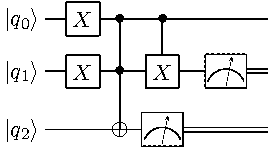
\includegraphics[width=0.6\textwidth]{figures/half-adder.pdf}
    \caption{Quantenschaltung f\"ur einen Halbaddierer}
  \end{figure}
\end{frame}

\section{Werkzeuge zur Implementierung}
\begin{frame}{Frametitle II}
  \begin{figure}[!h]
    \centering
    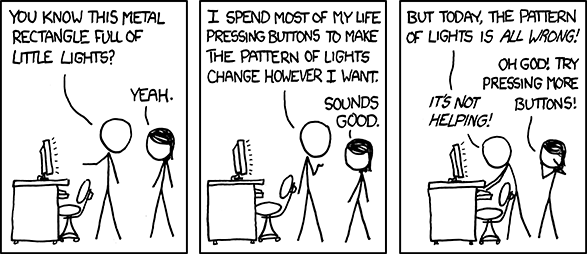
\includegraphics[width=0.7\textwidth]{figures/computer_problems.png}
  \end{figure}
\end{frame}
\begin{frame}
   Your text here \dots
\end{frame}
\begin{frame}
  Your text here \dots
\end{frame}

\section{Quantenalgorithmen}
\begin{frame}{The End}
  \begin{center}
    Thank you for your attention, are there any questions?
  \end{center}
\end{frame}

\section*{The End}
\begin{frame}[allowframebreaks]
  \frametitle{Literaturverzeichnis}
  \bibliographystyle{ieeetr}
  \bibliography{literature.bib}
\end{frame}

\end{document}

